\documentclass[sigconf]{acmart}

\input{format/final.tex}

\begin{document}
\title{Recipe Ingredient Analysis}


\author{Sushant Athaley}
\affiliation{%
  \institution{Indiana University}
}
\email{sathaley@iu.edu}

% The default list of authors is too long for headers}
\renewcommand{\shortauthors}{G. v. Laszewski}


\begin{abstract}
Food is the unavoidable part of day to day of human life. Ingredients play a major role or are the basic requirement in preparation of any kind of food. We can find the humongous list of ingredients getting used across globally along with other details which constitute to big data. We explore ingredients getting used in various recipes across the globe to understand most used ingredient, key ingredients of various cuisine and the relationship between the ingredients to find out closely related ingredients which can always provide great dish if used together.
\end{abstract}

\keywords{i523, hid302, big data, ingredient, recipe, analysis, python, gephi}

\maketitle

\section{Introduction}
Ingredients are vital for human existence as well as for food or restaurant industry. We use it every day for cooking and food industry uses it to produce consumable for their customers. Ingredient inspires chefs to come up with new culinary artistry. So what do we know about this essential element of the life and what data tell us? Ingredients come in different size, color, shape, flavor, nutrition, taste, texture, grows in specific weather conditions and this provides a great opportunity for various analysis which can be useful for the human being as well as business industries. So main focus of this study is on the ingredients used in various recipes across the cuisines. This study evaluates recipe ingredient dataset from Kaggle \cite{www-kaggle} to analyze most used ingredients, key cuisine ingredients and ingredient relationship.

This study is organized as follows, section \emph{Ingredient} defines ingredient and it's various characteristics. section \emph{Ingredeint Analytics} describes various analytics which can be performed on the ingredient with some examples. Section \emph{Project} describes the aim of this study. Section \emph{technologies} provides information on the tools and technologies used for this project. Section \emph{Methodology} covers overall process carried out in this project. Section \emph{Dataset} describes data structure used along with loading process and data findings. Section \emph{Analysis and Findings} describes various analysis carried out on the data and the visual representation of the analysis. Section \emph{Shortcomings} captures shortcomings of the project. Section \emph{Future Work} talks about what else can be done with this dataset which is not covered in the current scope of the project. Section \emph{Conclusion} concludes the study.  

\section{Ingredient}
Food is defined as ``Edible or potable substance (usually of animal or plant origin), consisting of nourishing and nutritive components such as carbohydrates, fats, proteins, essential mineral and vitamins, which (when ingested and assimilated through digestion) sustains life, generates energy, and provides growth, maintenance, and health of the body'' \cite{www-businessdictionary}. Thus food is the basic necessity for human for the sustainability. Food can be eaten raw, cooked or processed. As human race evolved over the period of time, the way we eat food is also evolved. Food cooking is just not the basic necessity but its an art and science in today's era. Food preparation consists of various cooking techniques, tools, and ingredients to make it palatable or edible by humans. The ingredient is by far the most important part of any food or recipe preparation. The recipe consists of the list of ingredients and the set of instruction to cook particular food dish \cite{www-collinsdictionary}. An ingredient is defined as ``Any of the foods or substances that are combined to make a particular dish'' \cite{www-oxforddictionaries}. Ingredients impart various flavors, aroma, texture, and color to the cooking dish. Ingredients are mostly derived from vegetables, fruits, nuts, grains, living organisms, herbs, flowers, and spices. It comes in both solid and liquid forms. Another characteristic of ingredients is the nutritional value they provide which is essential for the human body.

\section{Ingredient Analytics}
Ingredients characteristics and the combination of other related data provides various opportunities to analyze ingredient in different ways. Analysis of the flavors present in ingredient can provide us with the categorization of the different ingredient by the flavor profile which can be helpful in deciding substitute ingredient if a certain ingredient is not present or pairing ingredient from different flavor categories to construct the dish as per the taste required \cite{Ahn2011}. This analysis also helps to understand which ingredients cannot be used together. A similar analysis is carried out to correlate ingredient across recipes to come up with top 50 combinations of ingredients which can be used together \cite{www-r-bloggers}. Flavourspace application provides functionality to search recipe based on the ingredients, suggests alternate ingredient if not present, adjust the recipe as per the taste which is a good example of big data analytics in food industry \cite{www-thecul}. Foodpairing application takes another approach to form the connection between unfamiliar ingredients and provides information on how to use such ingredient to make a dish, this is very helpful in terms of sustainability as we can use ingredient which is ample available but not in use due to the absence of information on using such ingredients \cite{www-foodtech}.

Another study conducted on most used ingredient provides insight that sugar, oil, pepper, and salt are most commonly occurring ingredient, among spices clove, in vegetable onion,  garlic , and tomatoes, butter in milk product, eggs followed by chicken in the animal product are the most used ingredient in the categories \cite{Chatterjee2016}. This information can help in better planning and sourcing of such ingredients which are in high demand.

Ingredient nutrition analysis can help find out nutrition of the food prepared by those ingredients. This would be helpful in menu planning where nutrition information is the key factor such as school, hospitals or any other dietary program \cite{www-onlinelibrary}.

Recipe cost is calculated by including the cost of the ingredient used in that recipe. Ingredient cost as per the quantity used in recipe provides base information to calculate the price of any recipe. This ingredient cost analysis provides an avenue to reduce the cost of the recipe by using substitute ingredient of lesser cost. This can also help in household budget to keep in check as well as make restaurant industry profitable.

Ingredient used in recipe can provide insight into type of weather received by that cuisine as ingredient can grow in certain weather condition. This can help chef locally source the ingredient and maintain local agriculture sustainability.

\section{Project}
This project study is conducted to analyze ingredients getting used in various recipes across the cuisines to find out
\begin{itemize}
\item Most used ingredients across cuisines or globally
\item Key ingredients used by cuisines
\item Ingredient relationship or connection to understand the related ingredients
\end{itemize}

\subsection{Technologies}
Technologies and tools used in this projects are
\begin{itemize}
\item Python version 3.6 is used for data load and processing
\item Gephi 0.9.2 for visualization
\item Spyder 3.0 as a Python IDE
\end{itemize}

\subsection{Methodology}
The first step was to source the data. We were interested in the dataset which provides recipe information along with the ingredient used in the recipe. Since we wanted to analyze distribution across cuisines, data should also contain cuisine tagging. This dataset can be generated by pulling recipe data from various online applications or pick from publicly available datasets. We finalized publicly available dataset at Kaggle application satisfying need for this project.

Figure \ref{f:methodology} shows methodology used for this project to analyze ingredient data.
\begin{figure}[!ht]
  \centering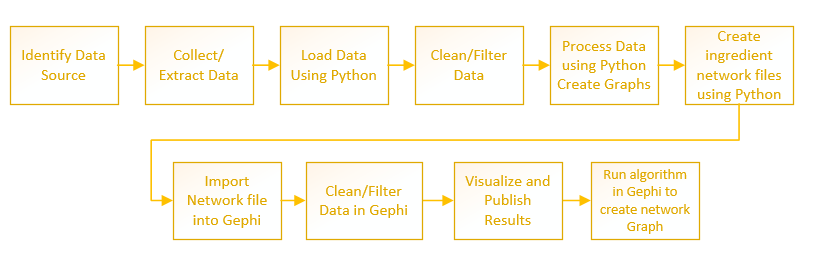
\includegraphics[width=\columnwidth]{images/methodology.PNG}
  \caption{Flowchart of the Methodology to Analyze Ingredients }\label{f:methodology}
\end{figure}

DataSet is loaded through Python script and further processed to clean the data. This cleaned data then processed to analyze ingredient distribution across cuisine and per cuisine. Gephi software is used to analyze the relationship and to find out the ingredient modularity. The Python script is used to create the network files required by the Gephi tool. Gephi requires Nodes and relationship in terms of Edges between the nodes for the analysis. The Python script is used to create Node and Edges file in excel format so that it can be imported into Gephi. Distinct ingredients used in recipe becomes the nodes. Edges or relationship between ingredients is derived by relating ingredients appearing in the same recipe. All ingredient in the same recipe is considered related to each other.
Network files created by Python are imported in Gephi to produce the graph for the visualization. Gephi tools data laboratory is used to clean up the data and filters are applied to provide usable network visualization. 

\subsection{Dataset}
The dataset for this study is sourced from Kaggle application \cite{www-kaggle}. This dataset is publicly available and featured in ``What's Cooking?'' competition. This dataset is in JSON format and of 12MB size. This dataset contains recipe id, cuisine and list of ingredients as described in Figure \ref{c:data-structure}.
\begin{figure}[htb]
\begin{verbatim}
{
 "id": 24717,
 "cuisine": "indian",
 "ingredients": [
     "tumeric",
     "vegetable stock",
     "tomatoes",
     "garam masala",
     "naan",
     "red lentils",
     "red chili peppers",
     "onions",
     "spinach",
     "sweet potatoes"
 ]
 },
\end{verbatim}
\caption{Ingredient Data Structure}\label{c:data-structure}
\end{figure}
This dataset contains total 39774 recipes across various cuisines. We used two different methods to load this data. Cuisine and ingredient analysis is done by loading data into \emph{pandas dataframe} and to analyze ingredient relationship data has been loaded into \emph{json} object. Figure \ref{c:data-loading} shows the code for data loading used in this project.
\begin{figure}[htb]
\begin{verbatim}
#read the ingredient data using pandas
dfTrain = pd.read_json('./data/train.json')


#load data using json
dataFilePath="./data/train.json"
with open(dataFilePath) as data_file:    
    data = json.load(data_file)
\end{verbatim}
\caption{Data Loading}\label{c:data-loading}
\end{figure}

Ingredient extraction from the data structure and processing was challenging as ingredients are listed comma separated for each recipe. Also, ingredient list can vary by recipe and there is no proper structure. Another issue with the ingredient list is ingredient appears in various forms but it's the same ingredient which gives duplicate data. For example, salt appears as salt, kosher salt, Morton Salt, sea salt, table salt, Himalayan salt, fine sea salt, low sodium salt, fine salt. This is the same ingredient but come across in recipe as a different ingredient and getting counted as a separate ingredient in the analysis. Some ingredients are listed along with measures like (10 oz.) frozen chopped spinach, (10 oz.) frozen chopped spinach, thawed and squeezed dry, (14.5 oz.) diced tomatoes and getting counted as a separate ingredient. Some ingredients are listed along with the brand name like KRAFT Reduced Fat Shredded Mozzarella Cheese, Johnsonville Smoked Sausage, Johnsonville Mild Italian Sausage Links etc and also constitutes to the ingredient list. This variation makes difficult to get the proper ingredient list for the analysis. Extensive work is needed to clean and correct the noisy data so that proper analysis can be carried out. This correction process is not carried out as part of this project.

Certain ingredients like salt or water etc should be avoided from the analysis as those are not the ingredient we are looking for the analysis. We tried to clean such elements during ingredient relationship analysis but we had little success as those ingredients are present in the dataset in various forms.  

\subsection{Analysis and Findings}

\subsubsection{Recipe Distribution By Cuisine}
We first analyze entire dataset to understand the total number of recipes and their distribution across various cuisines. We use Pythons Panda library to get the total recipe count as 39774 and plot the distribution. Figure \ref{f:Number_of_recipes_by_cuisine} shows number of recipes per cuisine. Dataset is heavily dominated by Italian cuisine followed by Mexican cuisine and with very fewer recipes from Russian and Brazilian cuisines. This also highlights another shortcoming of the dataset that it doesn't have equal representation of all cuisines which might give us biased analysis.
\begin{figure}[!ht]
  \centering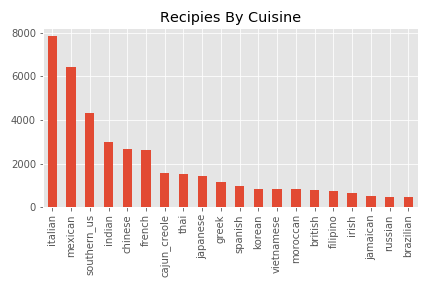
\includegraphics[width=\columnwidth]{images/Number_of_recipes_by_cuisine.png}
  \caption{Recipe Distribution By Cuisine }\label{f:Number_of_recipes_by_cuisine}
\end{figure}

Table\ref{t:recipecount} describes recipe count for every cuisine.
\begin{table}[htb]
\centering
\caption{Recipe Count By Cuisine}
\label{t:recipecount}
\begin{tabular}{ll}
Cuisine & Recipe Count \\
\hline
brazilian & 467 \\
british         &        804 \\
cajun creole    &       1546 \\
chinese         &       2673\\
filipino        &        755\\
french          &       2646\\
greek           &       1175\\
indian          &       3003\\
irish           &        667\\
italian         &       7838\\
jamaican        &        526\\
japanese        &       1423\\
korean          &        830\\
mexican         &       6438\\
moroccan        &        821\\
russian         &        489\\
southern us     &       4320\\
spanish         &        989\\
thai            &       1539\\
vietnamese      &        825\\

\end{tabular}
\end{table}

\subsubsection{Most Used Ingredients All Cuisines}
The second analysis is carried out to understand top 20 ingredients getting used across cuisine or globally. Ingredient \emph{Salt} is obvious topper followed by \emph{Oil} and \emph{Onions}. This also proves our craving for saltiness and fat. Figure \ref{f:Ingredient_Distribution} shows top 20 ingredient across cuisines. 
\begin{figure}[!ht]
  \centering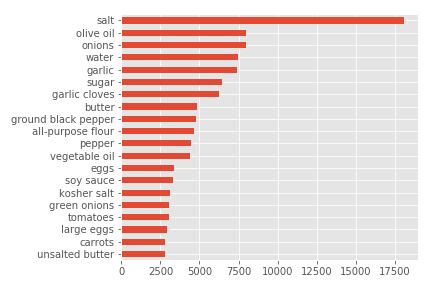
\includegraphics[width=\columnwidth]{images/Ingredient_Distribution.png}
  \caption{Top 20 Ingredients }\label{f:Ingredient_Distribution}
\end{figure}

\subsubsection{Ingredients Distribution By Cuisines}
The third analysis is carried out to understand key ingredient for each cuisine. These key ingredients define those cuisines and provide unique test characterized by that cuisine. We limited ingredient list to top 10 to get the key ingredients for each cuisine. Figure \ref{f:italian_10_most_used_ingredients}, \ref{f:brazilian_10_most_used_ingredients}, \ref{f:british_10_most_used_ingredients}, \ref{f:cajun_creole_10_most_used_ingredients}, \ref{f:chinese_10_most_used_ingredients}, \ref{f:filipino_10_most_used_ingredients}, \ref{f:french_10_most_used_ingredients}, \ref{f:greek_10_most_used_ingredients}, \ref{f:indian_10_most_used_ingredients}, \ref{f:irish_10_most_used_ingredients}, \ref{f:jamaican_10_most_used_ingredients}, \ref{f:japanese_10_most_used_ingredients}, \ref{f:korean_10_most_used_ingredients}, \ref{f:mexican_10_most_used_ingredients}, \ref{f:moroccan_10_most_used_ingredients}, \ref{f:russian_10_most_used_ingredients}, \ref{f:southern_us_10_most_used_ingredients}, \ref{f:spanish_10_most_used_ingredients}, \ref{f:thai_10_most_used_ingredients}, \ref{f:vietnamese_10_most_used_ingredients}  shows top 10 key ingredient used in the corresponding cuisines. 
\begin{figure}[!ht]
  \centering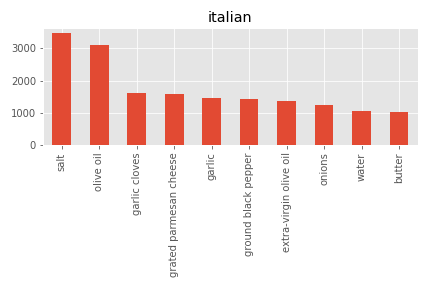
\includegraphics[width=\columnwidth]{images/italian_10_most_used_ingredients.png}
  \caption{Top 10 Ingredients }\label{f:italian_10_most_used_ingredients}
\end{figure}

\begin{figure}[!ht]
  \centering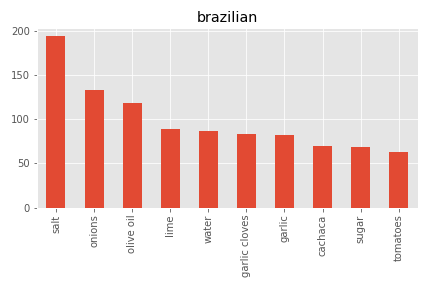
\includegraphics[width=\columnwidth]{images/brazilian_10_most_used_ingredients.png}
  \caption{Top 10 Ingredients }\label{f:brazilian_10_most_used_ingredients}
\end{figure}

\begin{figure}[!ht]
  \centering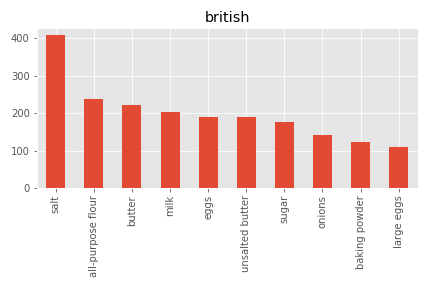
\includegraphics[width=\columnwidth]{images/british_10_most_used_ingredients.png}
  \caption{Top 10 Ingredients }\label{f:british_10_most_used_ingredients}
\end{figure}

\begin{figure}[!ht]
  \centering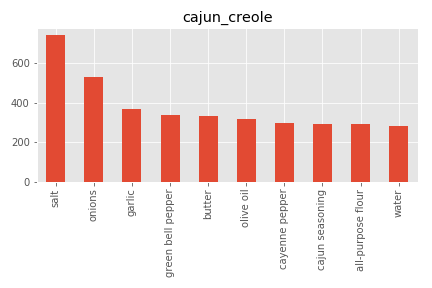
\includegraphics[width=\columnwidth]{images/cajun_creole_10_most_used_ingredients.png}
  \caption{Top 10 Ingredients }\label{f:cajun_creole_10_most_used_ingredients}
\end{figure}

\begin{figure}[!ht]
  \centering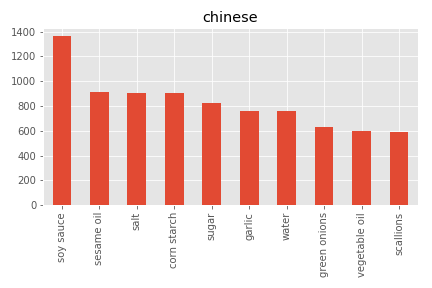
\includegraphics[width=\columnwidth]{images/chinese_10_most_used_ingredients.png}
  \caption{Top 10 Ingredients }\label{f:chinese_10_most_used_ingredients}
\end{figure}

\begin{figure}[!ht]
  \centering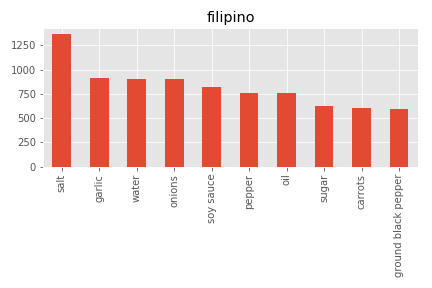
\includegraphics[width=\columnwidth]{images/filipino_10_most_used_ingredients.png}
  \caption{Top 10 Ingredients }\label{f:filipino_10_most_used_ingredients}
\end{figure}

\begin{figure}[!ht]
  \centering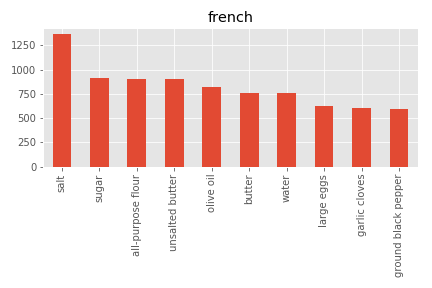
\includegraphics[width=\columnwidth]{images/french_10_most_used_ingredients.png}
  \caption{Top 10 Ingredients }\label{f:french_10_most_used_ingredients}
\end{figure}

\begin{figure}[!ht]
  \centering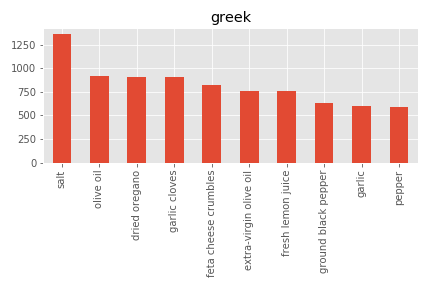
\includegraphics[width=\columnwidth]{images/greek_10_most_used_ingredients.png}
  \caption{Top 10 Ingredients }\label{f:greek_10_most_used_ingredients}
\end{figure}

\begin{figure}[!ht]
  \centering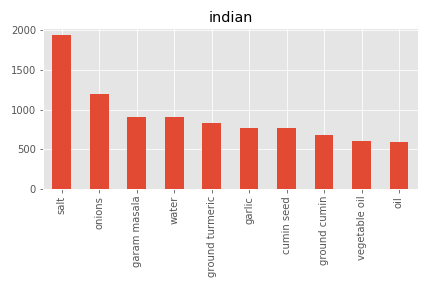
\includegraphics[width=\columnwidth]{images/indian_10_most_used_ingredients.png}
  \caption{Top 10 Ingredients }\label{f:indian_10_most_used_ingredients}
\end{figure}

\begin{figure}[!ht]
  \centering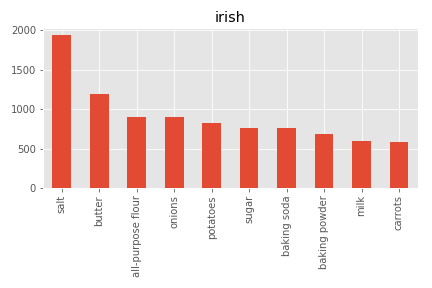
\includegraphics[width=\columnwidth]{images/irish_10_most_used_ingredients.png}
  \caption{Top 10 Ingredients }\label{f:irish_10_most_used_ingredients}
\end{figure}

\begin{figure}[!ht]
  \centering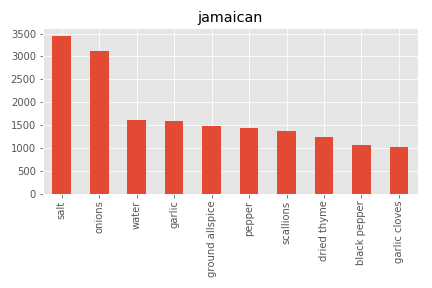
\includegraphics[width=\columnwidth]{images/jamaican_10_most_used_ingredients.png}
  \caption{Top 10 Ingredients }\label{f:jamaican_10_most_used_ingredients}
\end{figure}

\begin{figure}[!ht]
  \centering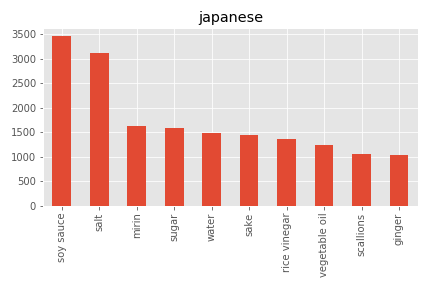
\includegraphics[width=\columnwidth]{images/japanese_10_most_used_ingredients.png}
  \caption{Top 10 Ingredients }\label{f:japanese_10_most_used_ingredients}
\end{figure}

\begin{figure}[!ht]
  \centering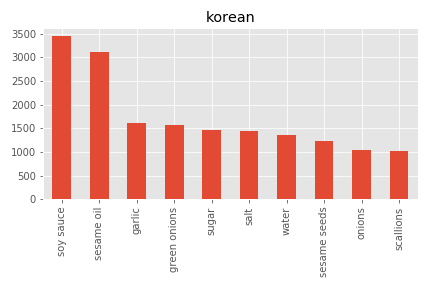
\includegraphics[width=\columnwidth]{images/korean_10_most_used_ingredients.png}
  \caption{Top 10 Ingredients }\label{f:korean_10_most_used_ingredients}
\end{figure}

\begin{figure}[!ht]
  \centering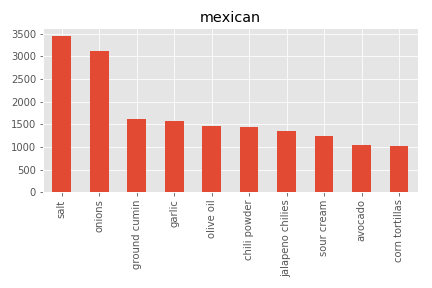
\includegraphics[width=\columnwidth]{images/mexican_10_most_used_ingredients.png}
  \caption{Top 10 Ingredients }\label{f:mexican_10_most_used_ingredients}
\end{figure}

\begin{figure}[!ht]
  \centering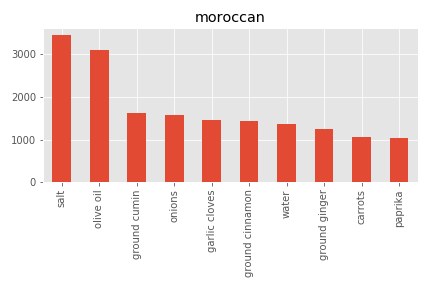
\includegraphics[width=\columnwidth]{images/moroccan_10_most_used_ingredients.png}
  \caption{Top 10 Ingredients }\label{f:moroccan_10_most_used_ingredients}
\end{figure}

\begin{figure}[!ht]
  \centering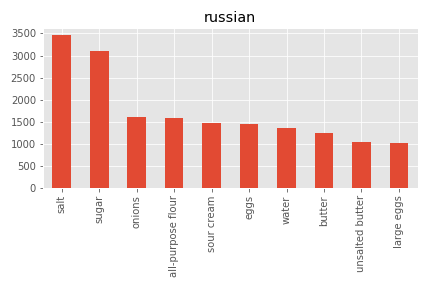
\includegraphics[width=\columnwidth]{images/russian_10_most_used_ingredients.png}
  \caption{Top 10 Ingredients }\label{f:russian_10_most_used_ingredients}
\end{figure}

\begin{figure}[!ht]
  \centering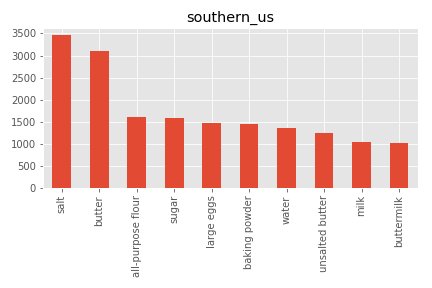
\includegraphics[width=\columnwidth]{images/southern_us_10_most_used_ingredients.png}
  \caption{Top 10 Ingredients }\label{f:southern_us_10_most_used_ingredients}
\end{figure}

\begin{figure}[!ht]
  \centering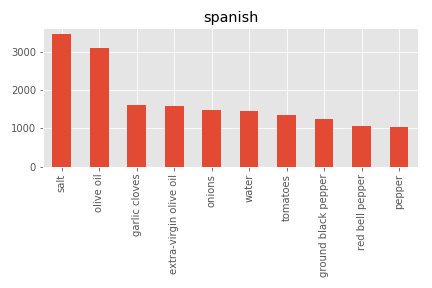
\includegraphics[width=\columnwidth]{images/spanish_10_most_used_ingredients.png}
  \caption{Top 10 Ingredients }\label{f:spanish_10_most_used_ingredients}
\end{figure}

\begin{figure}[!ht]
  \centering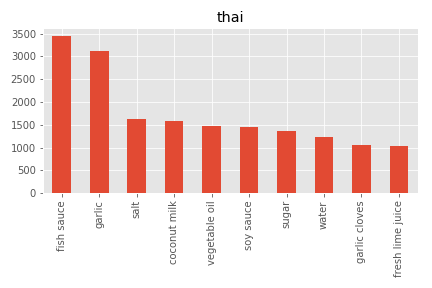
\includegraphics[width=\columnwidth]{images/thai_10_most_used_ingredients.png}
  \caption{Top 10 Ingredients }\label{f:thai_10_most_used_ingredients}
\end{figure}

\begin{figure}[!ht]
  \centering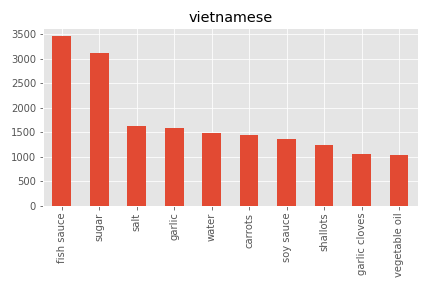
\includegraphics[width=\columnwidth]{images/vietnamese_10_most_used_ingredients.png}
  \caption{Top 10 Ingredients }\label{f:vietnamese_10_most_used_ingredients}
\end{figure}


\subsubsection{Ingredients Relationship}
Forth analysis is carried out to understand the relationship between the ingredient to find out ingredient clusters. This analysis helps us understand the ingredient combinations which can be used together to provide great dish every time. This model can be used to predict ingredients for certain recipe based on the cluster. We used Gephi tool to analyze and produce the graph for this analysis. Gephi accepts network structure in terms of Node and Edge relationship. We created this network using python by relating all ingredients present in the recipe with each other. Ingredients become the node and source and target nodes become the edges. These network files generated in excel spreadsheet are converted to CSV format and imported into the Gephi tool. Import created 5405 Nodes and 290828 edges for processing and analysis. Force Atlas 2 layout present in Gephi has been applied to the network which brings nodes with higher weights and shared connections closer to each other. We also used Gephi Data Laboratory to clean up duplicate or unwanted nodes. Filtering based on Degree Range and Edge Weight has been applied to data to reduce node and edges to get the graph which can be used for analysis and avoid crashing Gephi due to large data. Modularity statistic uncovered 5 ingredient clusters which can be identified by different color in the graph. This cluster can approximately related to the cuisines present in our dataset and confirms our earlier analysis of ingredient by cuisine.
\begin{itemize}
\item Orange - Mexican
\item Brown  - Indian
\item Blue   - Chinese
\item Green  - Italian
\item Gray   - Southern US
\end{itemize}

Figure \ref{f:ingredient_modularity} shows ingredient cluster of more than 1000 nodes. 
\begin{figure}[!ht]
  \centering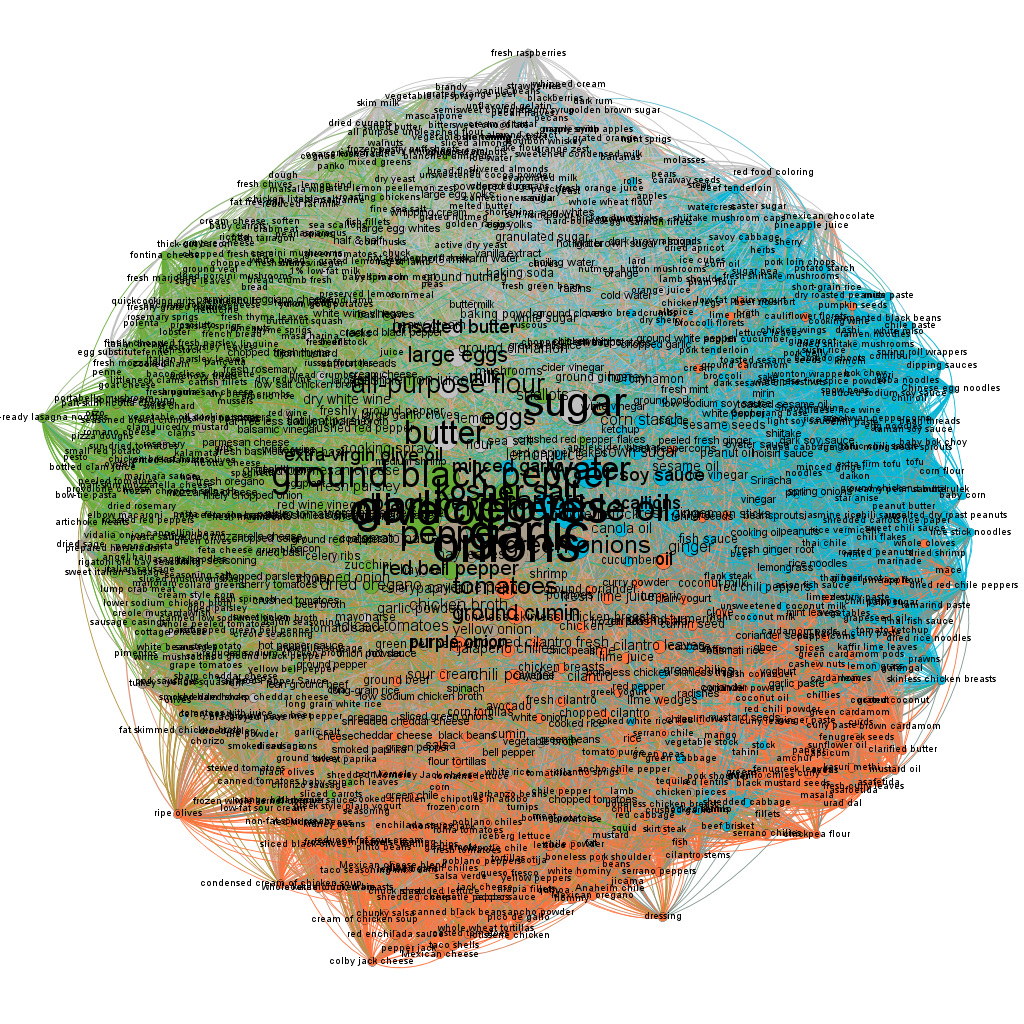
\includegraphics[width=\columnwidth]{images/ingredient_modularity.png}
  \caption{Ingredient Cluster }\label{f:ingredient_modularity}
\end{figure}

Figure \ref{f:ingredient_modularity100} shows ingredient cluster of around 100 nodes. 
\begin{figure}[!ht]
  \centering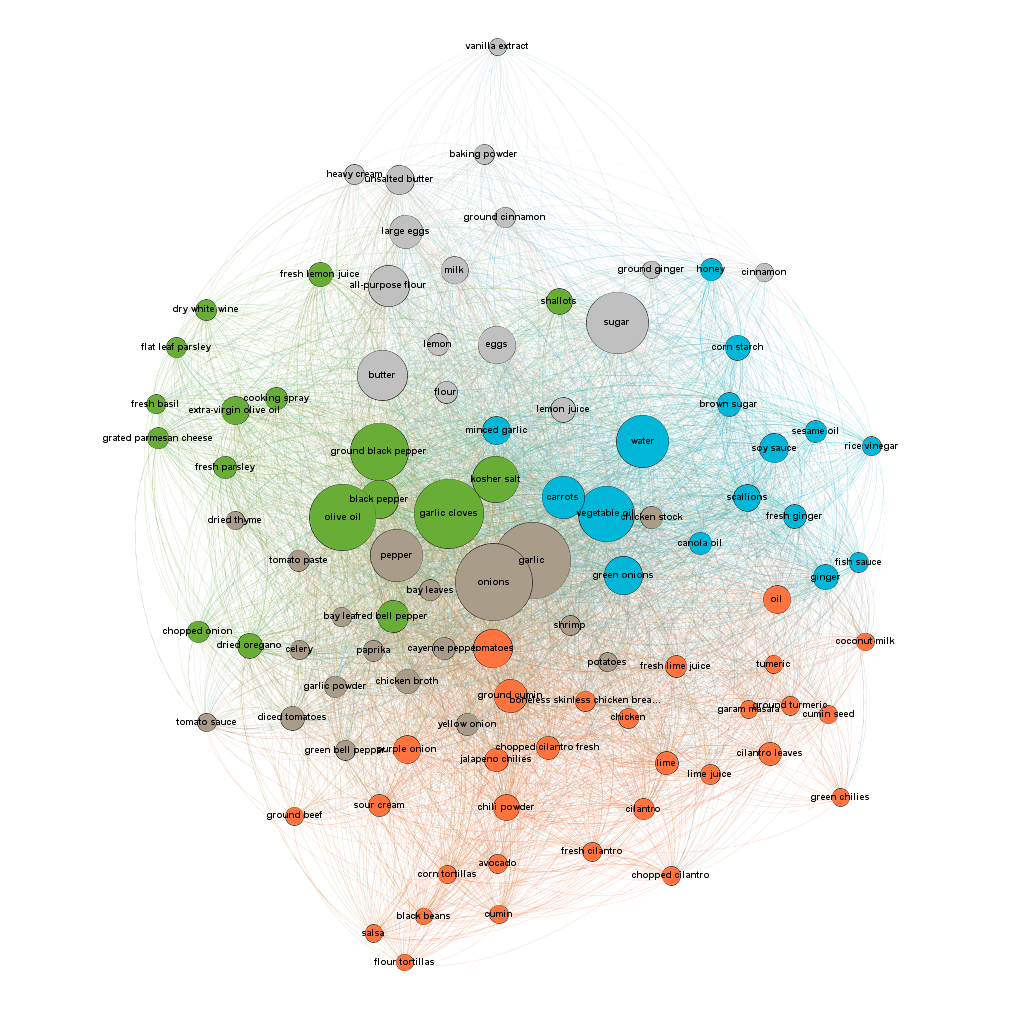
\includegraphics[width=\columnwidth]{images/ingredient_modularity100.png}
  \caption{ingredient Cluster 100 Nodes }\label{f:ingredient_modularity100}
\end{figure}

\subsection{Shortcomings}
Improper documentation of ingredient names in the dataset reduces the correctness of this analysis. In absence of proper ingredient name and duplication of ingredient name prevents getting exact ingredient weight into the analysis. A dataset with uniform ingredient name can help this analysis to achieve its best. If we don't find proper ingredient name then this analysis needs to include extensive data cleaning process which can be considered an improvement to this project.

Network file creation algorithm can be enhanced further by considering the number of recipes for the ingredient to provide additional weight to the relationship which can provide the stronger bond between the ingredients. 

\subsection{Future Work}
This dataset can be analyzed to find out ingredient overlap between various cuisine and can provide insight into the influence of one cuisine on another. Usually, geographically neighboring cuisines are influenced by each other as they share common ingredients.

\section{Conclusion}
This project shows most used ingredient, ingredient distribution by cuisine and predictive ingredient relationship model as per the goal of the project. We also show various opportunities present with ingredient data analysis and role of big data analytics. We prove human craving for salty and fatty food as salt and oil are most used ingredient across cuisines as per the analysis. We understand now based on our analysis key ingredient of any cuisine. Ingredient cluster shows why those ingredients are the base of certain cuisine and recipe of those ingredients always turn out delicious. We also crave for the good data so that we can provide more accurate analysis of the ingredients. Ingredient analysis has potential not only to help restaurant and food industry but it can help with our social responsibility of sustainability and understanding different cuisines and culture. As food industries interest grows in big data analytics, we will continue to see more evaluations of the ingredients.  

\begin{acks}
  The author would like to thank Dr. Gregor von Laszewski for his support and suggestions in this project. The author would also like to thank Kaggle application for hosting ingredient dataset which is used in this project and various online resource which helped understand Python and Gephi.  
\end{acks}

\bibliographystyle{ACM-Reference-Format}
\bibliography{report} 

\appendix

\input{issues}

\end{document}
